\section{Compiler intro}

\begin{figure}[h]
    \centering
    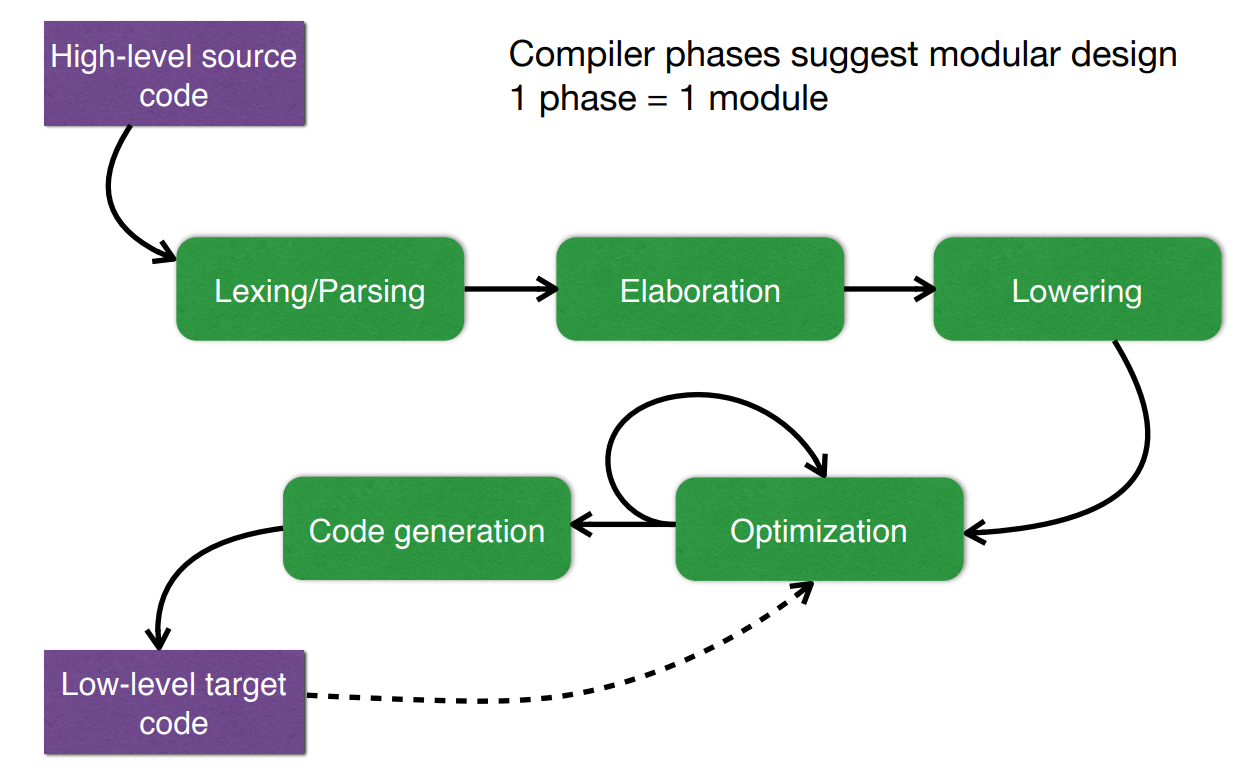
\includegraphics[scale=0.4]{assets/phases.png}
    \caption{Compiler modular phases.}
    \label{fig:phase}
\end{figure}

\begin{figure}[h]
    \centering
    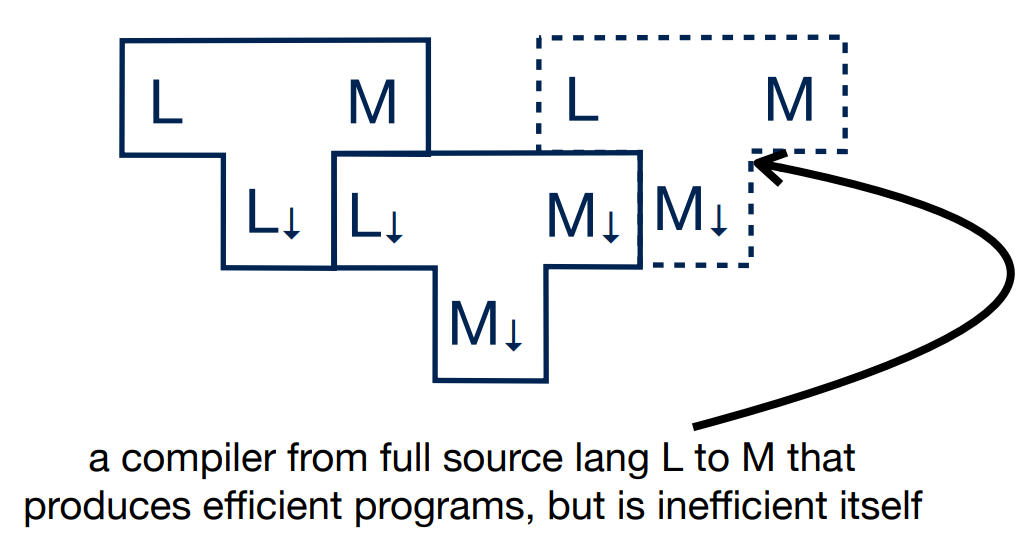
\includegraphics[scale=0.4]{assets/bootstrap_compile.png}
    \caption{Bootstrap compiling}
    \label{fig:bootstrap}
\end{figure}

\begin{itemize}
    \item \textbf{Lexing/Parsing}: String $\rightarrow_{lexing}$ Tokens $\rightarrow_{parsing}$ Abstract Syntax Tree (AST)
    \item \textbf{Elaboration}: \textit{Resolving scope }and \textit{Type checking}. Most errors found here.
    \item \textbf{Lowering}: High-level features to target-language like constructs (e.g. assembly-like). \textit{Intermediate representation}, LLVM.
    \item \textbf{Optimization}: Detect and rewrite expensive operations. Lifting invariants out of loops, parallelization.
    \item \textbf{Code generation}: fx LLVM to X86 (registers, instruction etc.)
    \item \textbf{Bootstrapping compilers}: Compile your language in your own language.
\end{itemize}